\documentclass{article}
	
\usepackage[margin=1in]{geometry}		% For setting margins
\usepackage{amsmath}				% For Math
\usepackage[]{amssymb}
\usepackage{amsmath}
\usepackage{gensymb}
\usepackage{fancyhdr}				% For fancy header/footer
\usepackage{graphicx}				% For including figure/image
\usepackage{cancel}					% To use the slash to cancel out stuff in work
\usepackage{wasysym}                % For cent symbol
\usepackage{needspace}              % To force item to next page

%%%%%%%%%%%%%%%%%%%%%%
% Set up fancy header/footer
\pagestyle{fancy}
\fancyhead[RO,R]{{\large\textbf{PHYS-102}}}
\fancyhead[LO,L]{\large{\textbf{Ch 19 Problem Set}}}
\fancyhead[CO,C]{\large{\textbf{Part 2}}}
% \fancyhead[RO,R]{\today}
\fancyfoot[LO,L]{}
\fancyfoot[CO,C]{\thepage}
\fancyfoot[RO,R]{}
\renewcommand{\headrulewidth}{0.4pt}
\renewcommand{\footrulewidth}{0.4pt}
%%%%%%%%%%%%%%%%%%%%%%

\newcommand{\hmwkTitle}{Chapter 19 Heat and the First Law of Thermodynamics}
% \newcommand{\hmwkDueDate}{February 12, 2014}
\newcommand{\hmwkClass}{PHYS-102}
% \newcommand{\hmwkClassTime}{}
% \newcommand{\hmwkClassInstructor}{Professor Isaac Newton}
\newcommand{\hmwkAuthorName}{\textbf{\underline{\hspace{3in}}}}

% math shortcuts
\newcommand\rr{\quad\Rightarrow\quad}

%
% Title Page
%

\title{
    \vspace{2in}
    \textmd{\textbf{\hmwkTitle}} \\
    \vspace{0.5in}
    \textmd{\textbf{\hmwkClass}}\\
    % \normalsize\vspace{0.1in}\small{Due\ on\ \hmwkDueDate\ at 3:10pm}\\
    % \vspace{0.1in}\large{\textit{\hmwkClassInstructor\ \hmwkClassTime}}
    \vspace{4in}
}

\author{\hmwkAuthorName}
\date{}
\begin{document}
\maketitle
% New blank page for printers that print on both sides of paper
% \clearpage\shipout\null
\begin{center}
    \section*{\textbf{\underline {Conceptual Questions}}}
\end{center}
    \subsection*{19. Explain in words why $C_P$ is greater than $C_V$.}
    \vspace{3in}
    \subsection*{20. Explain why the temperature of a gas increases when it is adiabatically compressed.}
\newpage
\clearpage\shipout\null
\begin{center}
    \section*{\textbf{\underline {Problems}}}
\end{center}
\noindent \large{\textbf{\textit{\underline{19-6 and 19-7  First Law of Thermodynamics}}}} \\
    \subsection*{27. Sketch a PV diagram of the following process: 2.0 L of ideal gas at atmospheric pressure are cooled at constant pressure to a volume of 1.0 L, and then expanded isothermally back to 2.0 L, whereupon the pressure is increased at constant volume until the original pressure is reached.}
    \vspace{3in}
    \subsection*{28. A gas is enclosed in a cylinder fitted with a light frictionless piston and maintained at atmospheric pressure. When 1250 kcal of heat is added to the gas, the volume is observed to increase slowly from 12.0 $m^3$ to 18.2 $m^3$. Calculate (a) the work done by the gas and (b) the change in internal energy of the gas.}
    \newpage
    \subsection*{29. The pressure in an ideal gas is cut in half slowly, while being kept in a container with rigid walls. In the process, 365 kJ of heat left the gas. (a) How much work was done during this process? (b) What was the change in internal energy of the gas during this process?}
    \vspace{3in}
    \subsection*{31. Consider the following two-step process. Heat is allowed to flow out of an ideal gas at constant volume so that its pressure drops from 2.2 atm to 1.4 atm. Then the gas expands at constant pressure, from a volume of 5.9 L to 9.3L, where the temperature reaches its original value. See Fig. 19–30. Calculate (a) the total work done by the gas in the process,
(b) the change in internal energy of the gas in the process, and (c) the total heat flow into or out of the gas.}
    \begin{figure*}[h]
            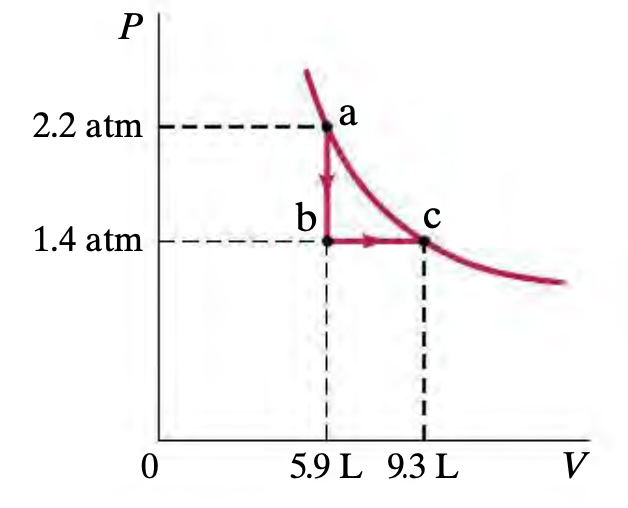
\includegraphics[width=0.4\textwidth]{figures/fig19-30.jpg}
    \end{figure*}
    \newpage
    \subsection*{32. The PV diagram in Fig. 19–31 shows two possible states of a system containing 1.55 moles of a monatomic ideal gas. $P_1$ = $P_2$ = 455 $N/m^2$, $V_1$ = 2.00 $m_3$, $V_2$ = 8.00 $m^3$. (a) Draw the process which depicts an isobaric expansion from state 1 to state 2, and label this process A. (b) Find the work done by the gas and the change in internal energy of the gas in process A. (c) Draw the two-step process which depicts an isothermal expansion from state 1 to the volume $V_2$, followed by an isovolumetric increase in temperature to
    state 2, and label this process B. (d) Find the change in internal energy of the gas for the two-step process B.}
    \begin{figure*}[h]
        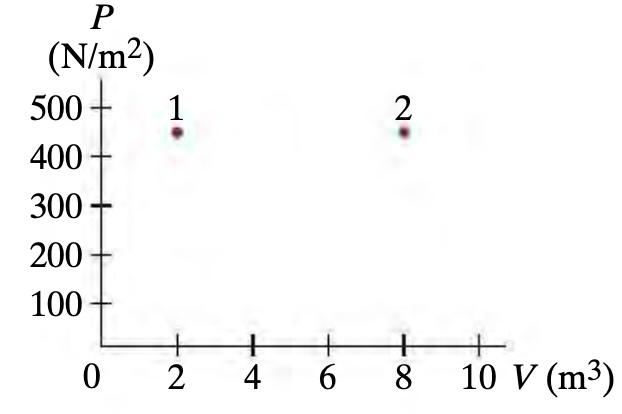
\includegraphics[width=0.45\textwidth]{figures/fig19-31.jpg}
    \end{figure*}
    \newpage
    \subsection*{33. Suppose 2.60mol of an ideal gas of volume $V_1$ = 3.50 $m^3$ at $T_1$ = 290K is allowed to expand isothermally to $V_2$ = 7.00 $m^3$ at $T_2$ = 290 K. Determine (a) the work done by the gas, (b) the heat added to the gas, and (c) the change in internal energy of the gas.}
    \vspace{3in}
    \subsection*{37. How much work is done by a pump to slowly compress, isothermally, 3.50 L of nitrogen at 0°C and 1.00 atm to 1.80 L at 0°C?}
    \newpage
    \noindent \large{\textbf{\textit{\underline{19-9 Adiabatic Expansion of a Gas}}}} \\
    \subsection*{51. A 1.00-mol sample of an ideal diatomic gas, originally at 1.00 atm and 20°C, expands adiabatically to 1.75 times its initial volume. What are the final pressure and temperature for the gas? (Assume no molecular vibration.)}
    \vspace{4in}
    \subsection*{52. Show, using Eqs. 19–6 and 19–15, that the work done by a gas that slowly expands adiabatically from pressure $P_1$ and Volume $V_1$, to $P_2$ and $V_2$, is given by}
    \[
        W = \displaystyle\frac{(P_1V_1 - P_2V_2)}{\lambda - 1}
    \]
    \newpage
    \subsection*{53. A 3.65-mol sample of an ideal diatomic gas expands adiabatically from a volume of 0.1210 $m^3$ to 0.750 $m^3$. Initially the pressure was 1.00 atm. Determine: (a) the initial and final temperatures; (b) the change in internal energy; (c) the heat lost by the gas; (d) the work done on the gas. (Assume no molecular vibration.)}
\end{document}
